\documentclass[12pt, titlepage]{article}
\usepackage[a4paper,margin=.75in]{geometry}
\usepackage{tgtermes}
\usepackage{amsmath}
\usepackage{setspace}
\usepackage{placeins}
\usepackage{listings}
\usepackage{color}
\usepackage{fancyhdr}
\usepackage{graphicx}
\usepackage[parfill]{parskip}
\usepackage{hyperref}
\hypersetup{
    colorlinks=true,
    linkcolor=blue,
    filecolor=magenta,      
    urlcolor=cyan,
}

\definecolor{dkgreen}{rgb}{0,0.6,0}
\definecolor{gray}{rgb}{0.5,0.5,0.5}
\definecolor{mauve}{rgb}{0.58,0,0.82}

\lstset{frame=none,
  language=Java,
  aboveskip=3mm,
  belowskip=3mm,
  showstringspaces=false,
  columns=flexible,
  basicstyle={\small\ttfamily},
  numbers=none,
  numberstyle=\tiny\color{gray},
  keywordstyle=\color{blue},
  commentstyle=\color{dkgreen},
  stringstyle=\color{mauve},
  breaklines=true,
  breakatwhitespace=true,
  tabsize=3
}

\pagestyle{fancyplain}
\lhead{Sean Connor}
\chead{Project 4 - Analysis}
\rhead{13 August 2018}

\title{Project 4 Analysis}
\author{Sean Connor \\ \\ 605.202 Data Structures \\ \\ 13 August 2018}
\date{}
\singlespacing

\begin{document}

\maketitle


\section {Data Structures}

The requirements defined for this project include the following:
\begin{itemize}
	\item Utilize Heap Sort to sort files of varying sizes/orders.
	\item Utilize Shell Sort with four different sets of gap values to sort files of varying sizes/orders.
	\item Analyze the performance of the different sorting algorithms and gap sizes by clocking time to sort completion.
	\item Both methods recursive or both methods iterative.
\end{itemize}

There are many ways to approach this project. The way I chose was to create a single class for each sort method for a total of two classes. Each class contained a main() driver method, with several other methods each to perform the tasks of reading the command line arguments to input file, converting the file data to array, and sorting, among others. There is no real advantage to using this approach - it was chosen without putting too much thought into deciding an ideal method. However, in retrospect I think it would be better to create separate classes for the sorts and for the driver. In the main driver class, one could simply instantiate a Sort object and call the required methods. This would be better for code reusability.

As far as the approaches to each sort, I chose to implement the Shell and Heap sorts iteratively and using an array. The justification for this is simple - I find iterative methods simpler to implement, they are more efficient in the majority of cases since one need not worry about the overhead associated with recursive methods, and the random access capability of arrays is ideal for performing many actions required for sorting. 

The ShellSort class contains a variety of methods - some that are necessary for sorting and some that are required for IO tasks. Some important methods are:
\begin{itemize}
	\item readFile(String filename, int size) - reads the input file and converts data to an int[] array.
	\item arrayToFile(int[] array, long time) - creates and returns a StringBuilder object with output values which can then be written using BufferedWriter. 
	\item sort(int[] data, int[] sequence) - iterates through the appropriate gap values and does an ``insertion sort'' at each gap value.
	\item insertionSort(int[] data, int gap) - performs an ``insertion sort'' using supplied gap value.
\end{itemize}

The HeapSort class contains a variety of methods - some that are necessary for sorting and some that are required for IO tasks. Some important methods are:
\begin{itemize}
	\item readFile(String filename, int size) - reads the input file and converts data to an int[] array.
	\item arrayToFile(int[] array, long time) - creates and returns a StringBuilder object with output values which can then be written using BufferedWriter. 
	\item heapify(int[] data, int index, int end) - rearrange the heap to maintain the heap property by swapping values so that parent node is always greater than child nodes.
	\item toMaxHeap(int[] data) - iterates through all parent nodes, calling heapify() to create a max heap.
	\item sort(int[] data) - creates a max heap, ``pulls off'' the top max value, places it at end of array, and then calls heapify to get the new max. This repeats until sorting is complete.
\end{itemize}




\section{General Strategy}

The input was read line by line from a text file using a combination of BufferedReader, InputStreamReader, and FileInputStream. The input text file must be formatted correctly, otherwise the program will produce an error message. A typical error is the inclusion of empty lines in the text file. The file is read line by line, with one integer value per line. Each value is placed in consecutive array index. With the file data in array format, the sorts can be performed.

The Shell Sort is essentially an optimized Insertion Sort. Shell Sort breaks a data set down into smaller pieces using a ``gap'' value and then sorts those pieces using a simple Insertion Sort. It iterates through smaller and smaller gap values until the gap = 1, and then the data set is sorted. Calling Shell Sort with single gap value of one is identical to Insertion Sort. Starting at array index 0+gap and iterating through until the end of the array, the data value at array[current] is compared to array[current-gap]. If array[current-gap] is larger, then the values will be swapped, and the process repeats until the swapped value is not greater than the preceding (by gap separation) value. 

Heap Sort relies upon the properties of a heap, that is that the parent is more ``extreme'' than its child nodes (meaning either greater than both child nodes or less than both child nodes). In this way, the root node of a heap will always be the largest or smallest value in the set. The root node can be ``removed'' from the heap, the heap is ``heapified'' to maintain the properties of a max or min heap, and the process repeats until the heap is empty and a complete sorted array has been created.

Finally, the data in the sorted array is appended to a StringBuilder object, which is returned and written to specified output file in the main() method using BufferedWriter/OutputStreamWriter/FileOutputStream.

When implementing both sorts, I consulted numerous sources, including the class lectures/notes, the Zybooks online textbook, and several web resources (see References section). 



\section{Algorithm Efficiency}

The time complexity of Shell Sort is not well defined, as the choice of gaps has a significant impact on efficiency. This is illustrated in Figures 1-4, where it is evident that the performance varies by choice of gaps. In the figures, Shell 1, Shell 2, and Shell 3 refer to the sequences required as per the assignment prompt. Shell 4 is a simple doubling sequence (1, 2, 4, 8, ..., 4096), and Shell 5 is a single gap value of one, which is essentially the same as a standard Insertion Sort. 

\begin{figure} [!htbp]
	\centering
	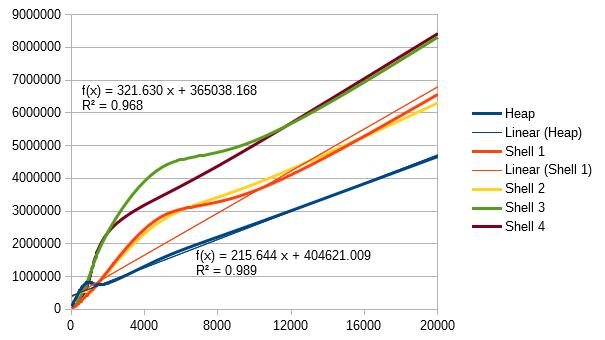
\includegraphics[width=5in]{ran-graph}
	\caption{Graph of time to sort unordered/random file (nanoseconds) versus number of items to be sorted.}
\end{figure}

\begin{figure} [!htbp]
	\centering
	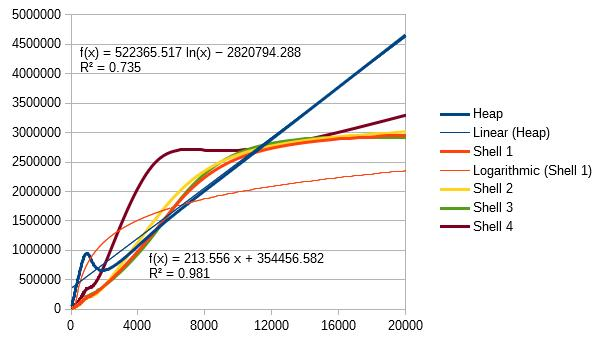
\includegraphics[width=5in]{asc-graph}
	\caption{Graph of time to sort ascending-order file (nanoseconds) versus number of items to be sorted.}
\end{figure}

\begin{figure} [!htbp]
	\centering
	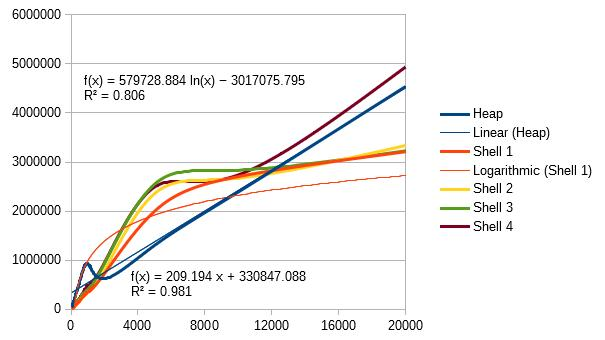
\includegraphics[width=5in]{rev-graph}
	\caption{Graph of time to sort reverse-ordered file (nanoseconds) versus number of items to be sorted.}
\end{figure}

\begin{figure} [!htbp]
	\centering
	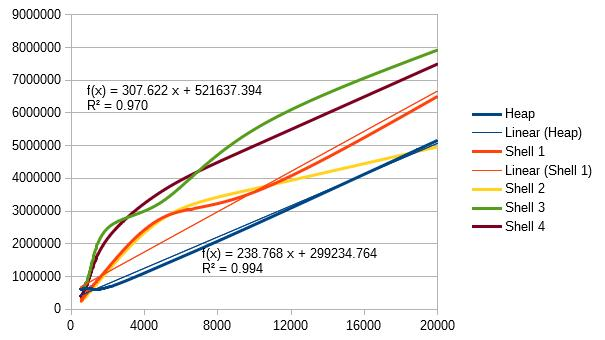
\includegraphics[width=5in]{dup-graph}
	\caption{Graph of time to sort file with multiple duplicates (nanoseconds) versus number of items to be sorted.}
\end{figure}

In general, the worst case time complexity of Shell Sort is between O(nlogn) and O(n\textsuperscript{2}), though using a linear trendline in LibreOffice resulted in decent R\textsuperscript{2} values for some cases (random, duplicates). Shell Sort with gap of one (Insertion Sort) has time complexity of O(n\textsuperscript{2}). Heap Sort time complexity is defined to be $\Omega$(nlogn), $\Theta$(nlogn), and O(nlogn) - the same performance in the best and worst case. See Figure 5 - Heap and Shell Sort are plotted against an nlogn function which clearly serves as an upper bound for values of n between 50 and 20000. The performance of Heap Sort is also plotted in Figures 1-4. In two cases, the performance of Heap Sort was better than Shell Sort (random, duplicates), while in the other two cases (ascending, reversed) the time to completion using Shell Sort came to a relative plateau and was more efficient at higher values of n. However relatively speaking, the performance of the two is very similar. A better illustration of this can be seen in Figures 6 and 7.

\begin{figure} [!htbp]
	\centering
	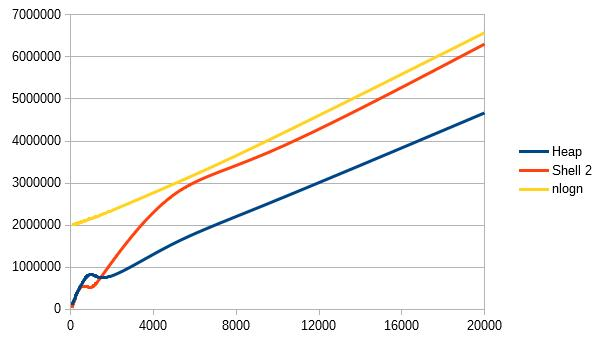
\includegraphics[width=5in]{nlogn}
	\caption{A plot of a constant times nlog\textsubscript{2}n plus a constant (16nlog\textsubscript{2}n+2000000) against Heap Sort and Shell 2.}
\end{figure}

Shell 5 (Insertion Sort) is compared to Heap Sort and Shell 2 in Figures 6 and 7. Additional figures are included in the Appendix. For all cases but one (ascending/nearly sorted), and performance of Insertion Sort was substantially worse than Shell Sort and Heap Sort. This is not surprising, as the best case performance of Insertion Sort is $\Omega$(n) for nearly sorted sets and $\Theta$(n\textsuperscript{2}) and O(n\textsuperscript{2}) for other cases.


\begin{figure} [!htbp]
	\centering
	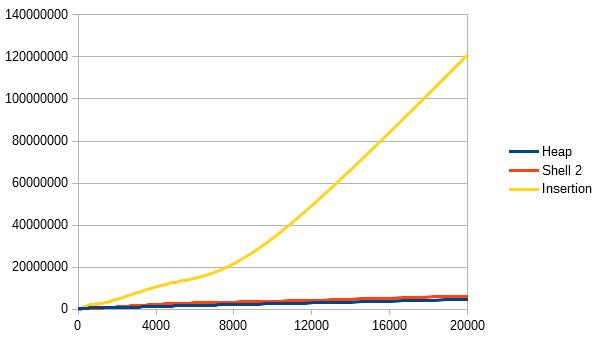
\includegraphics[width=5in]{ran2}
	\caption{Graph of time to sort unordered/random file (nanoseconds) versus number of items to be sorted.}
\end{figure}

\begin{figure} [!htbp]
	\centering
	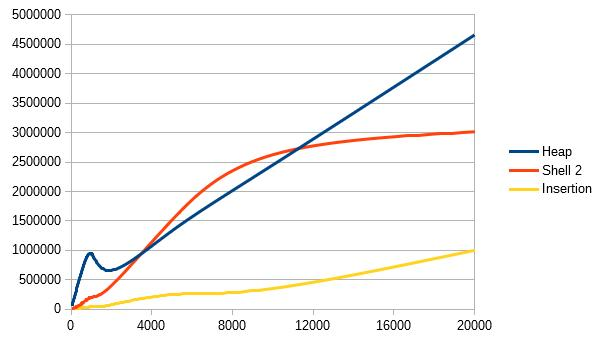
\includegraphics[width=5in]{asc2}
	\caption{Graph of time to sort ascending-order file (nanoseconds) versus number of items to be sorted.}
\end{figure}

All in all, it seems that Heap Sort and Shell Sort (assuming a good gap sequence) are good choices for sorting for any data set (sorted, unsorted, duplicates, etc). Shell Sort seems to have a slight edge with nearly-sorted or reverse-sorted files, while Heap Sort performs better with random/unsorted files. In both cases, the worst case space complexity is O(1), as no additional overhead is required, and array indices are simply manipulated/swapped. If one has no idea as to the sorted status of data, either Heap Sort or Shell Sort would be a good choice; however, if one knows that the data is nearly sorted, then simple Insertion Sort has a best case performance of $\Omega$(n), which is better than either Heap Sort or Shell Sort. For Shell Sort, sequence 1 (Knuth's sequence) performed well in all cases, and so would be a solid choice for any Shell Sort implementation.

The sorted status of the data has the greatest effect on efficiency if one considers the change in performance from ascending order file to random file for Insertion Sort. If Insertion Sort is not a consideration, then the gap sequence of Shell Sort has the most substantial effect on efficiency.

\section{Lessons Learned}
As mentioned previously, I think that a recursive implementation of either Shell Sort or Heap Sort would not be as efficient. This is primarily from the overhead associated with recursion, which I suspect would be more significant as the size of the file increases. However, from NIST's Dictionary of Algorithms and Data Structures the definition of heapify is to ``rearrange a heap to maintain the heap property, that is, the key of the root node is more extreme (greater or less) than or equal to the keys of its children. If the root node's key is not more extreme, swap it with the most extreme child key, then recursively heapify that child's subtree. The child subtrees must be heaps to start.'' While I personally find the iterative method simpler to implement and visualize, I can understand how a recursive method could be an elegant solution.

I'm a firm believer in the idea that people learn best by \textit{doing}. That is certainly the case here. My initial attempts at implementing Heap Sort were not going great, and so I consulted the internet. Through the process of attempting a solution and then seeing how it could be done better I gain a better perspective of overall programming paradigms.
 

\newpage

\section{References}
\begin{enumerate}
	\item Johns Hopkins University 605.202 Data Structures Lectures and Online Textbook
	\item ``Priority Queues'' Algorithms 4th Ed. \url{https://algs4.cs.princeton.edu/24pq/}
	\item ``Heapify All The Things With Heap Sort'' Medium.com. \url{https://medium.com/basecs/heapify-all-the-things-with-heap-sort-55ee1c93af82}
	\item ``heapify'' NIST Dictionary of Algorithms and Data Structures. \url{https://xlinux.nist.gov/dads/HTML/heapify.html}
	\item ``Know Thy Complexities'' Big-O Cheatsheet. \url{http://bigocheatsheet.com/}	
\end{enumerate}

\newpage

\section{Appendix}

\begin{figure} [!htbp]
	\centering
	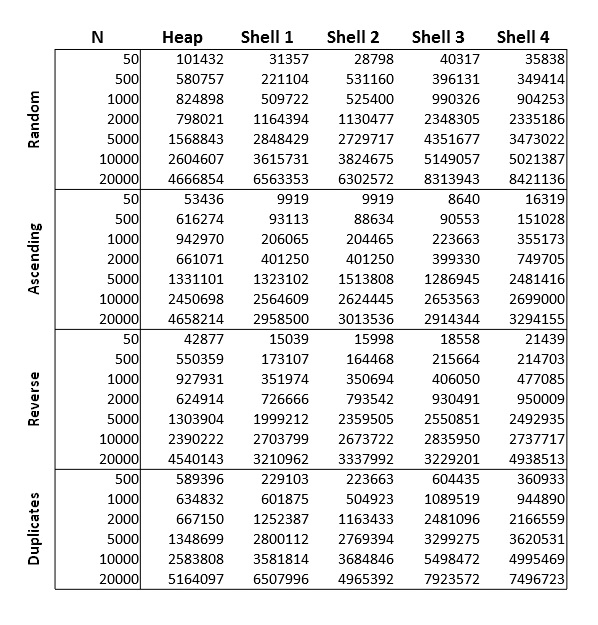
\includegraphics[width=5in]{Performance}
	\caption{Table of time to completion results (in nanoseconds) for various file orders/sizes. Only one run of each was performed (i.e. results are not averaged over several runs). Note that even the slowest case still completed in less than a hundredth of a second.}
\end{figure}

\begin{figure} [!htbp]
	\centering
	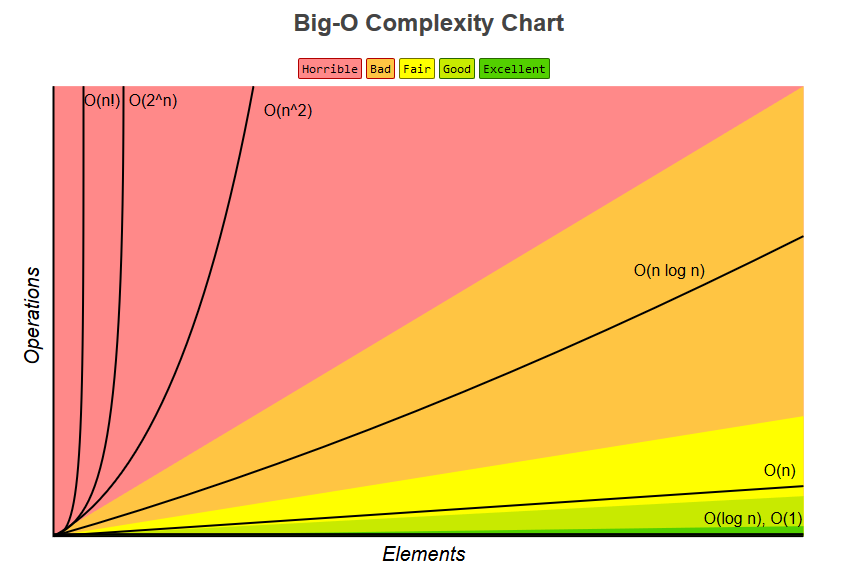
\includegraphics[width=4in]{complexity}
	\caption{Complexity graph}
\end{figure}

\newpage

\begin{figure} [!htbp]
	\centering
	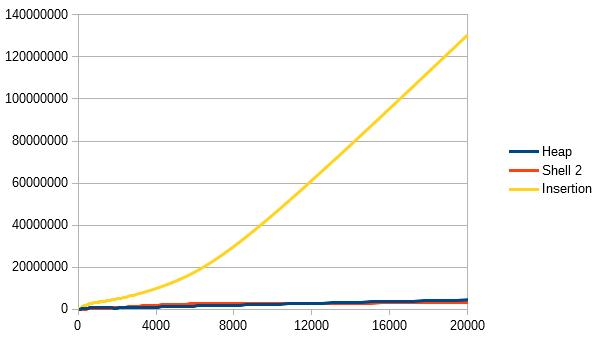
\includegraphics[width=5in]{rev2}
	\caption{Graph of time to sort reverse-ordered file (nanoseconds) versus number of items to be sorted.}
\end{figure}

\begin{figure} [!htbp]
	\centering
	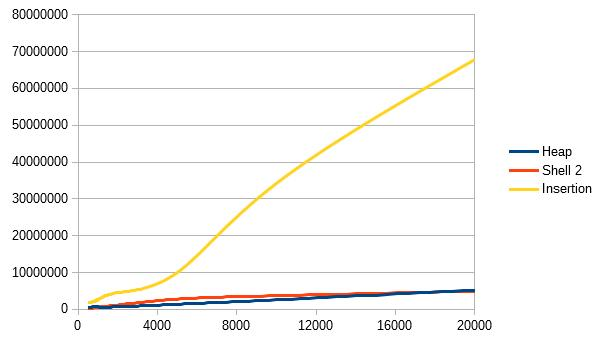
\includegraphics[width=5in]{dup2}
	\caption{Graph of time to sort file with multiple duplicates (nanoseconds) versus number of items to be sorted.}
\end{figure}

\end{document}